\documentclass[
%% TIKZ_CLASSOPTION %%
tikz
]{standalone}
\usepackage{amsmath}
\usetikzlibrary{matrix}
%% EXTRA_TIKZ_PREAMBLE_CODE %%
\begin{document}
%% TIKZ_CODE %%
\tikzset{every picture/.style={line width=2.5pt}} %set default line width to 0.75pt
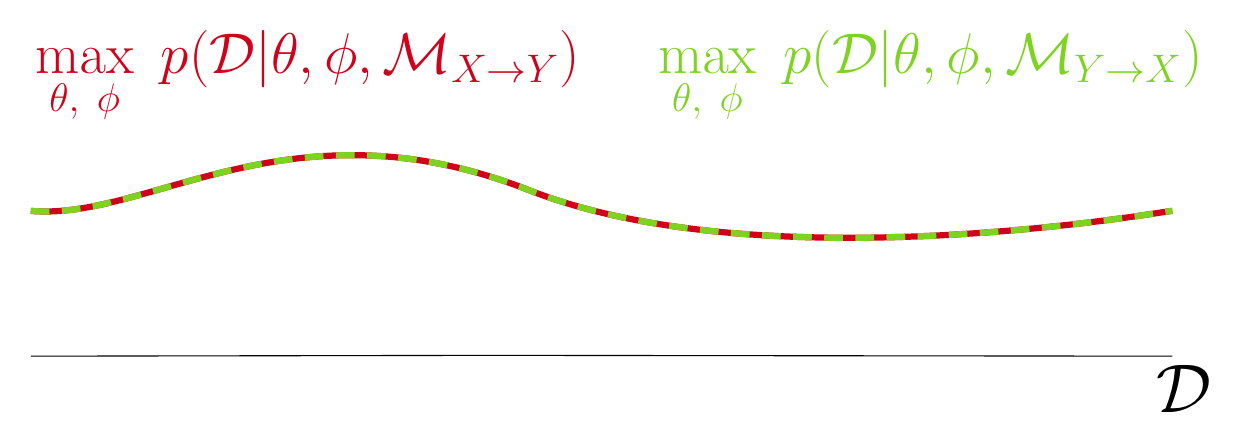
\begin{tikzpicture}[x=0.75pt,y=0.75pt,yscale=-1,xscale=1]
%uncomment if require: \path (0,300); %set diagram left start at 0, and has height of 300

%Straight Lines [id:da7493139746626474]
\draw    (50,180) -- (272,179.61) -- (600,180) ;
%Curve Lines [id:da8407783790065078]
\draw [color={rgb, 255:red, 208; green, 2; blue, 27 }  ,draw opacity=1 ][line width=2.25]    (50,110) .. controls (107,115) and (175,55) .. (290,100) .. controls (405,145) and (596.71,109.94) .. (600,110) ;
%Curve Lines [id:da7678987550251666]
\draw [color={rgb, 255:red, 126; green, 211; blue, 33 }  ,draw opacity=1 ][line width=2.25]  [dash pattern={on 6.75pt off 4.5pt}]  (50,110) .. controls (107,115) and (175,55) .. (290,100) .. controls (405,145) and (596.71,109.94) .. (600,110) ;

% Text Node
\draw (591,183) node [anchor=north west][inner sep=0.75pt]  [font=\Huge] [align=left] {$\displaystyle \mathcal{D}$};
% Text Node
\draw (51,22) node [anchor=north west][inner sep=0.75pt]  [font=\huge,color={rgb, 255:red, 208; green, 2; blue, 27 }  ,opacity=1 ] [align=left] {$\displaystyle \max_{\theta ,\ \phi } \ p(\mathcal{D} |\theta ,\phi ,\mathcal{M}_{X\rightarrow Y})$};
% Text Node
\draw (351,22) node [anchor=north west][inner sep=0.75pt]  [font=\huge,color={rgb, 255:red, 126; green, 211; blue, 33 }  ,opacity=1 ] [align=left] {$\displaystyle \max_{\theta ,\ \phi } \ p(\mathcal{D} |\theta ,\phi ,\mathcal{M}_{Y\rightarrow X})$};
\end{tikzpicture}
\end{document}
